% Created: 2013-09-24
\documentclass[english]{../thermomemo/thermomemo}
\usepackage[T1]{fontenc}
\usepackage[utf8]{inputenc}
\usepackage{siunitx}
\usepackage{amsfonts,amsmath,amsthm,amssymb}
\usepackage{hyperref}
\usepackage{cleveref}
\usepackage{pgfplots}
\usepackage{tikz}
\usepackage{color}
\usepackage{url}
\usepackage{graphicx}
\usepackage[bf,small,margin=10pt]{caption}
\usepackage[margin=1em]{subcaption}
\usepackage{bm}
\usepackage{booktabs}
\usepackage[numbers]{natbib}

\definecolor{urlblue}{RGB}{70,130,180}
\hypersetup{
  colorlinks=true,
  linkcolor=black,
  urlcolor=urlblue,
  citecolor=black,
}

% TikZ and pgfplots
\usetikzlibrary{arrows}
\pgfplotsset{
  compat=1.6,
  width=0.8\textwidth,
  grid=major,
  every axis legend/.append style={
    at={(0,1.02)},
    anchor=south west,
  },
  every axis plot/.style={
    black,
    solid,
    thick,
  },
  legend cell align=left,
  legend style={column sep=0.5em,draw=white},
  xlabel={$T\;[\si{K}]$},
  ylabel={$p\;[\si{bar}]$},
}

\newcommand{\myplotNL}[2]{
  \addplot[#1] file[skip first] {data/#2.dat};
}

\newcommand{\myplot}[3]{
  \addplot[#1] file[skip first] {data/#2.dat};
  \addlegendentry{#3}
}

\crefname{equation}{Eq.}{Eqs.}
\crefname{section}{Section}{Sections}
\crefname{chapter}{Chapter}{Chapters}
\crefname{figure}{Figure}{Figures}
\crefname{subfigure}{Figure}{Figures}
\crefname{table}{Table}{Tables}

\title{Documentation of the binary-XY code in thermopack}
\author{Morten Hammer}
\date{\today}

\graphicspath{{gfx/}}

% Fancy differential from Claudio Beccari, TUGboat
% * No need for manual tweak of spaces.
% * Copied from Svend Tollak Munkejord.
\makeatletter
\newcommand*{\dif}{\@ifnextchar^{\DIfF}{\DIfF^{}}}
\def\DIfF^#1{\mathop{\mathrm{\mathstrut d}}\nolimits^{#1}\gobblesp@ce}
\def\gobblesp@ce{\futurelet\diffarg\opsp@ce}
\def\opsp@ce{%
  \let\DiffSpace\!%
  \ifx\diffarg(%
    \let\DiffSpace\relax
  \else
    \ifx\diffarg[%
      \let\DiffSpace\relax
    \else
      \ifx\diffarg\{%
        \let\DiffSpace\relax
      \fi\fi\fi\DiffSpace}
\makeatother

% New commands
\newcommand*{\ifrac}[2]{\ensuremath{#1/#2}}
\newcommand*{\volume}{V}
\newcommand*{\area}{A}
\newcommand*{\volumeint}[1]{\ensuremath{\int_{\volume}#1\dif\volume}}
\newcommand*{\areaint}[1]{\ensuremath{\int_{\area}#1\dif\area}}
\newcommand*{\dt}[1]{\ensuremath{\frac{\dif #1}{\dif t}}}
\newcommand*{\dti}[1]{\ifrac{\dif #1}{\dif t}}
\newcommand*{\pdt}[1]{\ensuremath{\frac{\partial #1}{\partial t}}}
\newcommand*{\pdti}[1]{\ifrac{\partial #1}{\partial t}}
\newcommand*{\td}[2]{\frac{\mathrm{d} #1}{\mathrm{d} #2}}
\newcommand*{\tdi}[1]{\mathrm D #1 /\mathrm Dt}
\newcommand*{\od}[2]{\ensuremath{\frac{\dif#1}{\dif{#2}}}}
\newcommand*{\odi}[2]{\ensuremath{{\dif#1}/{\dif{#2}}}}
\newcommand*{\pd}[2]{\ensuremath{\frac{\partial #1}{\partial{#2}}}}
\newcommand*{\pdi}[2]{\ensuremath{{\partial #1}/{\partial{#2}}}}
\newcommand*{\vct}[1]{\ensuremath{\boldsymbol{#1}}}
\newcommand*{\normal}{\ensuremath{\vct n}}
\renewcommand*{\div}{\boldsymbol\nabla\cdot}
\newcommand*{\divs}{\boldsymbol\nabla_{\text s}\cdot}
\newcommand*{\grad}{\boldsymbol\nabla}
\newcommand*{\grads}{\boldsymbol\nabla_{\text s}}
\newcommand*{\lapl}{\boldsymbol\Delta}
\newcommand*{\lapls}{\boldsymbol\Delta_{\text s}}
\newcommand*{\sint}[2]{\ensuremath{\int_{#1}#2\dif #1}}
\newcommand*{\surint}[2]{\ensuremath{\int_{#1}#2\dif S}}
\newcommand*{\chr}{\chi}
\newcommand*{\bigo}[1]{\ensuremath{\mathcal{O}\left(#1\right)}}
\newcommand*{\smallo}[1]{\ensuremath{o\left(#1\right)}}
\newcommand*{\eint}[1]{\ensuremath{\int_{-\infty}^\infty #1\dif z}}
\newcommand*{\zint}[1]{\ensuremath{\int #1\dif z}}
\newcommand*{\ejmp}[1]{\ensuremath{\left[#1\right]_{-\infty}^\infty}}
\newcommand*{\zlimp}{\ensuremath{\lim_{z\to\infty}}}
\newcommand*{\zlimm}{\ensuremath{\lim_{z\to-\infty}}}
\newcommand*{\zlimpm}{\ensuremath{\lim_{z\to\pm\infty}}}
\newcommand*{\ndot}{\ensuremath{\vct n\cdot}}
\newcommand*{\vext}{\ensuremath{V_{\text{ext}}}}
\newcommand*{\txin}{\ensuremath{\textup{in}\ }}
\newcommand*{\txon}{\ensuremath{\textup{on}\ }}
\newcommand{\spec}{\text{spec}}
\newcommand{\coto}{\ensuremath{\text{CO}_{\text{\scriptsize 2}}}}
\newcommand{\no}{\ensuremath{\text{NO}}}
\newcommand{\CO}{CO\ensuremath{_2}}
\newcommand{\N}{N\ensuremath{_2}}
\newcommand{\thermo}{\textsc{Thermopack}}
\newcommand{\TPlib}{\textsc{TPlib}}

\newcommand*{\out}{\ensuremath{\text{out}}}
\newcommand*{\ideal}{\ensuremath{\text{ideal}}}
\newcommand*{\recovery}{\ensuremath{\text{recovery}}}
\newcommand*{\capture}{\ensuremath{\text{capture}}}

\begin{document}

\frontmatter

\tableofcontents

\clearpage

\section{Introduction}
The equations required to describe an binary Txy or Pxy plot.

\section{Governing equations}
\label{sec:eqn}
The equation system $\mathbf{F(X)}=\mathbf{0}$, is defined by equation
\eqref{eq:fug_eq} to \eqref{eq:X}.
\begin{align}
 f_i  & = \ln K_i + \ln \hat{\varphi}_i\left(\mathbf{y}\right)- \ln
 \hat{\varphi}_i\left(\mathbf{x}\right) = 0, \quad
 i=1,2 \label{eq:fug_eq} \\
 f_{i+2}  & = y_i - K_i x_i = 0, \quad i=1,2 \label{eq:k_eq} \\
 f_{5}  & = x_1 + x_2 - 1 = 0 \label{eq:x_eq} \\
 f_{6}  & = y_1 + y_2 - 1 = 0 \label{eq:y_eq} \\
 f_{7}  & = S - S_{\spec} = 0 \label{eq:spec_eq} \\
\end{align}

\begin{equation}
\label{eq:F}
 \mathbf{F} = \begin{pmatrix}
          f_1 \\
          \vdots \\
          f_7
\end{pmatrix}
\end{equation}

The last variable will be $\ln T$ or $\ln P$, for simplicity the
equations are written out for a Txy binary plot. The temperature is
therefore constant. The last variable is therefore $\ln P$. The Pxy
problem can be developed in the same manner.   
\begin{equation}
\label{eq:X}
 \mathbf{X} = \begin{pmatrix}
          \ln \mathbf{K} \\
          \mathbf{x} \\
          \mathbf{y} \\
          \ln P
\end{pmatrix}
\end{equation}

% \nomenclature[mu]{$\mathbf{u}$}{Variable vector}
% \nomenclature[mb]{$\mathbf{B}$}{Nonconservative flux matrix}
% \nomenclature[mf]{$\mathbf{F}$}{Flux function}
% \nomenclature[ms]{$\mathbf{s}$}{Source function}
% \nomenclature[mw]{$\mathbf{w}$}{Nonconservative flux}
% \nomenclature[ah]{$h$}{Enthalpy}

\subsection{Changing the specification}
Differentiating, we get:
\begin{align}
\td{\mathbf{F(X)}}{\mathbf{X}}\td{\mathbf{X}}{S_{\spec}} 
+\td{\mathbf{F(X)}}{S_{\spec}} &= \mathbf{0}\\
\td{\mathbf{F(X)}}{\mathbf{X}}\td{\mathbf{X}}{S_{\spec}} 
 = \begin{pmatrix} \mathbf{0}\\
1
\end{pmatrix}
\end{align}

We are therefore able to produce new initial guesses when we change
the specification, $S_{\spec}$.

\subsection{Termination}
The binaryXY routine need to terminate when one of the following
situations occur:
\begin{enumerate}
\item One of the components become zero.
\item Critical point or azeotrope is
  reached. ($\mathbf{x}=\mathbf{y}$) \label{enum:crit}
\item User given maximum in pressure or minimum in temperature is reached. \label{enum:temp} 
\end{enumerate}

\section{Results}
Have tested the mixture \coto-\no~with SRK and PR. Both have been
tested with the binary interaction parameters $k_{ij}=0$ and
$k_{ij}=-0.105$. The plots have been initialised at the \coto~bubble point.

See Figure \ref{fig:srk_0}, \ref{fig:srk_opt}, \ref{fig:pr_0} and \ref{fig:pr_opt}.
\begin{figure}[tbp]
  \centering
  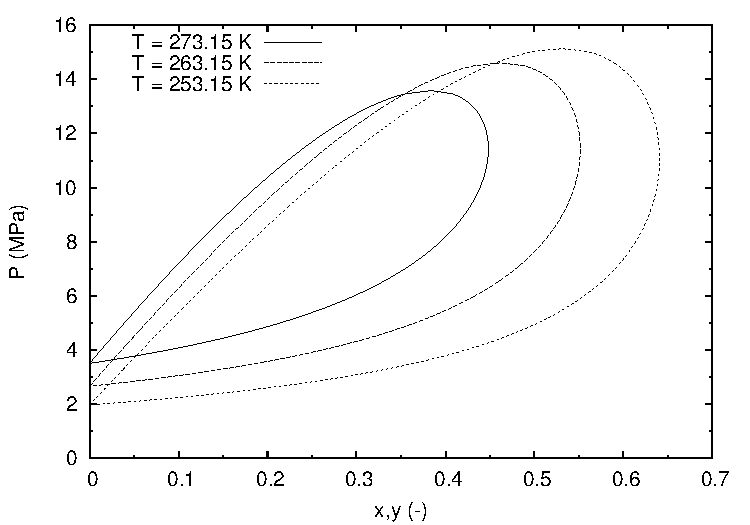
\includegraphics[width=0.8\textwidth]{NO_SRK_Txy_k0.pdf}
  \caption{Mole fraction of \no~in an\coto-\no~mixture with SRK and $k_{ij}=0$.}
  \label{fig:srk_0}
\end{figure}

\begin{figure}[tbp]
  \centering
  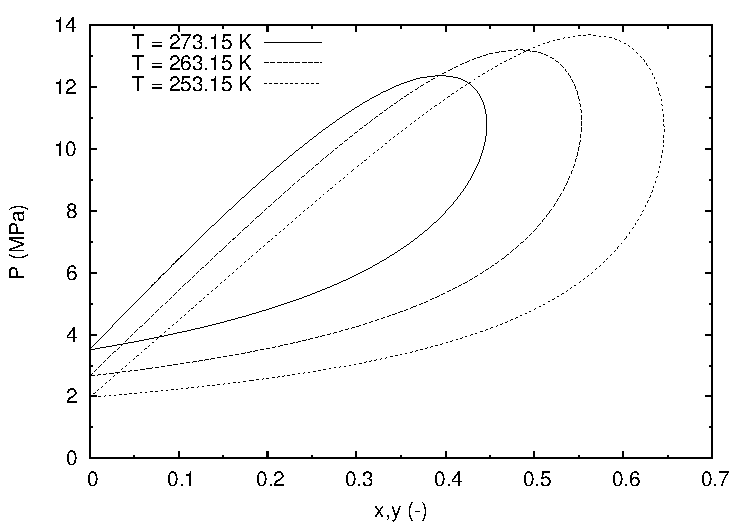
\includegraphics[width=0.8\textwidth]{NO_SRK_Txy.pdf}
  \caption{Mole fraction of \no~in an\coto-\no~mixture with SRK and $k_{ij}=-0.119$.}
  \label{fig:srk_opt}
\end{figure}

\begin{figure}[tbp]
  \centering
  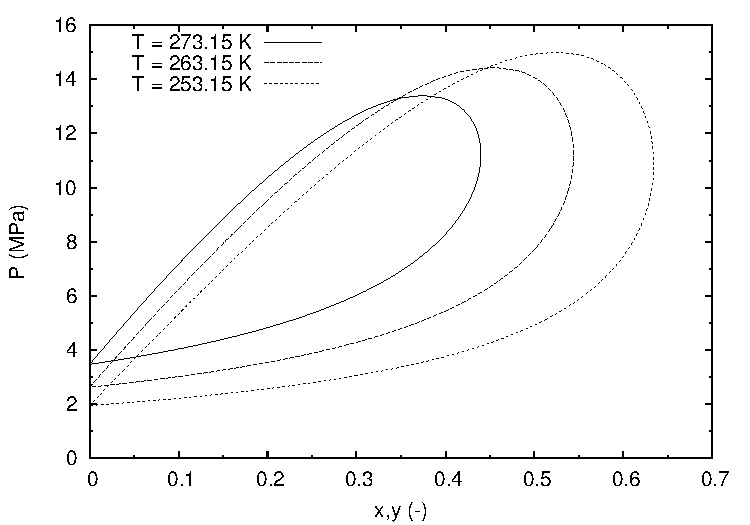
\includegraphics[width=0.8\textwidth]{NO_PR_Txy_k0.pdf}
  \caption{Mole fraction of \no~in an\coto-\no~mixture with PR and $k_{ij}=0$.}
  \label{fig:pr_0}
\end{figure}

\begin{figure}[tbp]
  \centering
  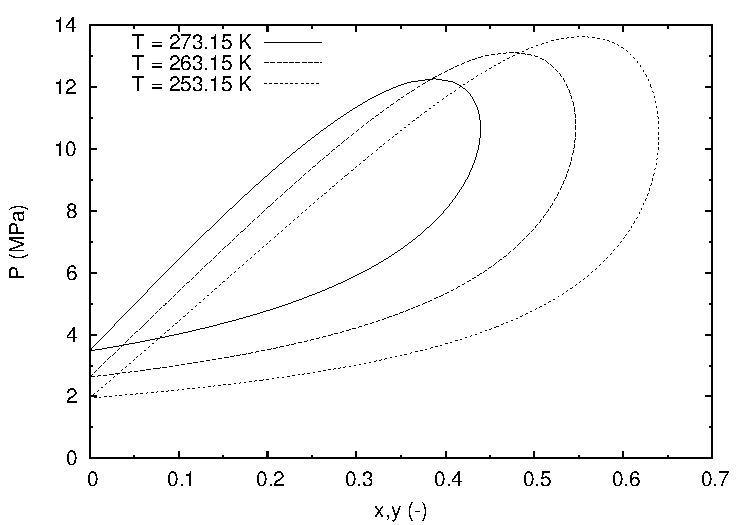
\includegraphics[width=0.8\textwidth]{NO_PR_Txy.pdf}
  \caption{Mole fraction of \no~in an\coto-\no~mixture with PR and $k_{ij}=-0.105$.}
  \label{fig:pr_opt}
\end{figure}

\appendix

\section{Jacobian}
The Jacobian required for a Newton solver of the equation system in
section \ref{sec:eqn}.

\begin{align}
 \pd{f_1}{\ln K_1}  & = 1 \\
 \pd{f_1}{\ln K_2}  & = 0 \\
 \pd{f_1}{x_i}  & =  - \pd{\ln
 \hat{\varphi}_1\left(\mathbf{x}\right)}{x_i}, \quad
 i=1,2\\
 \pd{f_1}{y_i}  & =  \pd{\ln
 \hat{\varphi}_1\left(\mathbf{y}\right)}{y_i}, \quad
 i=1,2\\
 \pd{f_1}{\ln P}  & =  P\left(\pd{\ln
 \hat{\varphi}_1\left(\mathbf{y}\right)}{P} -\pd{\ln
 \hat{\varphi}_1\left(\mathbf{x}\right)}{P}\right)
\end{align}

\begin{align}
 \pd{f_2}{\ln K_1}  & = 0 \\
 \pd{f_2}{\ln K_2}  & = 1 \\
 \pd{f_2}{x_i}  & =  - \pd{\ln
 \hat{\varphi}_2\left(\mathbf{x}\right)}{x_i}, \quad
 i=1,2\\
 \pd{f_2}{y_i}  & =  \pd{\ln
 \hat{\varphi}_2\left(\mathbf{y}\right)}{y_i}, \quad
 i=1,2\\
 \pd{f_2}{\ln P}  & =  P\left(\pd{\ln
 \hat{\varphi}_2\left(\mathbf{y}\right)}{P} -\pd{\ln
 \hat{\varphi}_2\left(\mathbf{x}\right)}{P}\right)
\end{align}

\begin{align}
 \pd{f_3}{\ln K_1}  & = -K_1 x_1 \\
 \pd{f_3}{\ln K_2}  & = 0 \\
 \pd{f_3}{x_1}  & =  - K_1 \\
 \pd{f_3}{x_2}  & = 0 \\
 \pd{f_3}{y_1}  & = 1 \\
 \pd{f_3}{y_2}  & = 0 \\
 \pd{f_3}{\ln P}  & = 0
\end{align}

\begin{align}
 \pd{f_4}{\ln K_1}  & = 0 \\
 \pd{f_4}{\ln K_2}  & = -K_2 x_2 \\
 \pd{f_4}{x_1}  & = 0\\
 \pd{f_4}{x_2}  & = - K_2 \\
 \pd{f_4}{y_1}  & = 0 \\
 \pd{f_4}{y_2}  & = 1 \\
 \pd{f_4}{\ln P}  & = 0
\end{align}

\begin{align}
 \pd{f_5}{X_i}  & = 0 \quad i=1,2,5,6,7\\
 \pd{f_5}{x_i}  & = 1 \quad i=3,4
\end{align}

\begin{align}
 \pd{f_6}{X_i}  & = 0 \quad i=1,2,3,4,7\\
 \pd{f_6}{y_i}  & = 1 \quad i=5,6
\end{align}

\begin{equation}
 \pd{f_7}{X_i} =\begin{cases} 1 & i=i_{\spec}\\
   0 & \text{otherwise}
\end{cases}
\end{equation}

\end{document}
